
%-----------------------------------------------------------------------------------------------------------------------------------------------%
%	The MIT License (MIT)
%
%	Copyright (c) 2021 Philip Empl
%
%	Permission is hereby granted, free of charge, to any person obtaining a copy
%	of this software and associated documentation files (the "Software"), to deal
%	in the Software without restriction, including without limitation the rights
%	to use, copy, modify, merge, publish, distribute, sublicense, and/or sell
%	copies of the Software, and to permit persons to whom the Software is
%	furnished to do so, subject to the following conditions:
%	
%	THE SOFTWARE IS PROVIDED "AS IS", WITHOUT WARRANTY OF ANY KIND, EXPRESS OR
%	IMPLIED, INCLUDING BUT NOT LIMITED TO THE WARRANTIES OF MERCHANTABILITY,
%	FITNESS FOR A PARTICULAR PURPOSE AND NONINFRINGEMENT. IN NO EVENT SHALL THE
%	AUTHORS OR COPYRIGHT HOLDERS BE LIABLE FOR ANY CLAIM, DAMAGES OR OTHER
%	LIABILITY, WHETHER IN AN ACTION OF CONTRACT, TORT OR OTHERWISE, ARISING FROM,
%	OUT OF OR IN CONNECTION WITH THE SOFTWARE OR THE USE OR OTHER DEALINGS IN
%	THE SOFTWARE.
%	
%
%-----------------------------------------------------------------------------------------------------------------------------------------------%


%============================================================================%
%
%	DOCUMENT DEFINITION
%
%============================================================================%

\documentclass[10pt,A4,english]{article}	


%----------------------------------------------------------------------------------------
%	ENCODING
%----------------------------------------------------------------------------------------

% we use utf8 since we want to build from any machine
\usepackage[utf8]{inputenc}		
\usepackage[USenglish]{isodate}
\usepackage{fancyhdr}
\usepackage[numbers]{natbib}

%----------------------------------------------------------------------------------------
%	LOGIC
%----------------------------------------------------------------------------------------

% provides \isempty test
\usepackage{xstring, xifthen}
\usepackage{enumitem}
\usepackage[english]{babel}
\usepackage{blindtext}
\usepackage{pdfpages}
\usepackage{changepage}
%----------------------------------------------------------------------------------------
%	FONT BASICS
%----------------------------------------------------------------------------------------

% some tex-live fonts - choose your own

% \usepackage[defaultsans]{droidsans}
%\usepackage[default]{comfortaa}
%\usepackage{cmbright}
\usepackage[default]{raleway}
% \usepackage{fetamont}
%\usepackage[default]{gillius}
%\usepackage[light,math]{iwona}
% \usepackage[thin]{roboto}

% set font default
\renewcommand*\familydefault{\sfdefault} 	
\usepackage[T1]{fontenc}

% more font size definitions
\usepackage{moresize}

%----------------------------------------------------------------------------------------
%	FONT AWESOME ICONS
%---------------------------------------------------------------------------------------- 

% include the fontawesome icon set
\usepackage{fontawesome}

% use to vertically center content
% credits to: http://tex.stackexchange.com/questions/7219/how-to-vertically-center-two-images-next-to-each-other
\newcommand{\vcenteredinclude}[1]{\begingroup
\setbox0=\hbox{\includegraphics{#1}}%
\parbox{\wd0}{\box0}\endgroup}
\newcommand{\tab}[1]{\hspace{.2\textwidth}\rlap{#1}}
% use to vertically center content
% credits to: http://tex.stackexchange.com/questions/7219/how-to-vertically-center-two-images-next-to-each-other
\newcommand*{\vcenteredhbox}[1]{\begingroup
\setbox0=\hbox{#1}\parbox{\wd0}{\box0}\endgroup}

% icon shortcut
\newcommand{\icon}[3] { 							
	\makebox(#2, #2){\textcolor{maincol}{\csname fa#1\endcsname}}
}	


% icon with text shortcut
\newcommand{\icontext}[4]{ 						
	\vcenteredhbox{\icon{#1}{#2}{#3}}  \hspace{2pt}  \parbox{0.9\mpwidth}{\textcolor{#4}{#3}}
}

% icon with website url
\newcommand{\iconhref}[5]{ 						
    \vcenteredhbox{\icon{#1}{#2}{#5}}  \hspace{2pt} \href{#4}{\textcolor{#5}{#3}}
}

% icon with email link
\newcommand{\iconemail}[5]{ 						
    \vcenteredhbox{\icon{#1}{#2}{#5}}  \hspace{2pt} \href{mailto:#4}{\textcolor{#5}{#3}}
}

%----------------------------------------------------------------------------------------
%	PAGE LAYOUT  DEFINITIONS
%----------------------------------------------------------------------------------------

% page outer frames (debug-only)
% \usepackage{showframe}		

% we use paracol to display breakable two columns
\usepackage{paracol}
\usepackage{tikzpagenodes}
\usetikzlibrary{calc}
\usepackage{lmodern}
\usepackage{multicol}
\usepackage{lipsum}
\usepackage{atbegshi}
% define page styles using geometry
\usepackage[a4paper]{geometry}

% remove all possible margins
\geometry{top=1cm, bottom=1cm, left=1cm, right=1cm}

\usepackage{fancyhdr}
\pagestyle{empty}

% space between header and content
% \setlength{\headheight}{0pt}

% indentation is zero
\setlength{\parindent}{0mm}

%----------------------------------------------------------------------------------------
%	TABLE /ARRAY DEFINITIONS
%---------------------------------------------------------------------------------------- 

% extended aligning of tabular cells
\usepackage{array}

% custom column right-align with fixed width
% use like p{size} but via x{size}
\newcolumntype{x}[1]{%
>{\raggedleft\hspace{0pt}}p{#1}}%


%----------------------------------------------------------------------------------------
%	GRAPHICS DEFINITIONS
%---------------------------------------------------------------------------------------- 

%for header image
\usepackage{graphicx}

% use this for floating figures
% \usepackage{wrapfig}
% \usepackage{float}
% \floatstyle{boxed} 
% \restylefloat{figure}

%for drawing graphics		
\usepackage{tikz}			
\usepackage{ragged2e}	
\usetikzlibrary{shapes, backgrounds,mindmap, trees}

%----------------------------------------------------------------------------------------
%	Color DEFINITIONS
%---------------------------------------------------------------------------------------- 
\usepackage{transparent}
\usepackage{color}

% primary color
\definecolor{maincol}{RGB}{64,64,64}

% accent color, secondary
% \definecolor{accentcol}{RGB}{ 250, 150, 10 }

% dark color
\definecolor{darkcol}{RGB}{70,70,70}

% light color
\definecolor{lightcol}{RGB}{245,245,245}

\definecolor{accentcol}{RGB}{59,77,97}



% Package for links, must be the last package used
\usepackage[hidelinks]{hyperref}

% returns minipage width minus two times \fboxsep
% to keep padding included in width calculations
% can also be used for other boxes / environments
\newcommand{\mpwidth}{\linewidth-\fboxsep-\fboxsep}
	


%============================================================================%
%
%	CV COMMANDS
%
%============================================================================%

%----------------------------------------------------------------------------------------
%	 CV LIST
%----------------------------------------------------------------------------------------

% renders a standard latex list but abstracts away the environment definition (begin/end)
\newcommand{\cvlist}[1] {
	\begin{itemize}{#1}\end{itemize}
}

%----------------------------------------------------------------------------------------
%	 CV TEXT
%----------------------------------------------------------------------------------------

% base class to wrap any text based stuff here. Renders like a paragraph.
% Allows complex commands to be passed, too.
% param 1: *any
\newcommand{\cvtext}[1] {
	\begin{tabular*}{1\mpwidth}{p{0.98\mpwidth}}
		\parbox{1\mpwidth}{#1}
	\end{tabular*}
}
\newcommand{\cvtextsmall}[1] {
	\begin{tabular*}{0.8\mpwidth}{p{0.8\mpwidth}}
		\parbox{0.8\mpwidth}{#1}
	\end{tabular*}
}
%----------------------------------------------------------------------------------------
%	CV SECTION
%----------------------------------------------------------------------------------------

% Renders a a CV section headline with a nice underline in main color.
% param 1: section title
\newcommand{\cvsection}[1] {
	\vspace{14pt}
	\cvtext{
		\textbf{\LARGE{\textcolor{darkcol}{#1}}}\\[-4pt]
		\textcolor{accentcol}{ \rule{0.2\textwidth}{1.5pt} } \\
	}
}

\newcommand{\cvsectionskill}[1] {
	\vspace{14pt}
	\cvtext{
		\textbf{\LARGE{\textcolor{darkcol}{#1}}}\textbf{\small{\textcolor{darkcol}{\hspace{18}(0 to 5 yrs.)}}}\\[-4pt]
		\textcolor{accentcol}{ \rule{0.2\textwidth}{1.5pt} } \\
	}
}

\newcommand{\cvsectionsmall}[1] {
	\vspace{10pt}
	\cvtext{
		\textbf{\fontsize{13}{10}\selectfont{\textcolor{darkcol}{#1}}}\\[-6pt]
		\textcolor{accentcol}{ \rule{0.2\textwidth}{1.5pt} } \\
	}
}

\newcommand{\cvheadline}[1] {
	\vspace{16pt}
	\cvtext{
		\textbf{\Huge{\textcolor{accentcol}{#1}}}\\[-4pt]
		 
	}
}

\newcommand{\cvsubheadline}[1] {
	\vspace{16pt}
	\cvtext{
		\textbf{\huge{\textcolor{darkcol}{#1}}}\\[-4pt]
		 
	}
}
%----------------------------------------------------------------------------------------
%	META SKILL
%----------------------------------------------------------------------------------------

% Renders a progress-bar to indicate a certain skill in percent.
% param 1: name of the skill / tech / etc.
% param 2: level (for example in years)
% param 3: percent, values range from 0 to 1
\newcommand{\cvskill}[3] {
	\begin{tabular*}{1\mpwidth}{p{0.72\mpwidth}  r}
 		\textcolor{black}{\textbf{#1}} & \textcolor{maincol}{#2}\\
	\end{tabular*}%
	
	\hspace{4pt}
	\begin{tikzpicture}[scale=1,rounded corners=2pt,very thin]
		\fill [lightcol] (0,0) rectangle (1\mpwidth, 0.15);
		\fill [accentcol] (0,0) rectangle (#3\mpwidth, 0.15);
  	\end{tikzpicture}%
	\\[-8pt]%
}


%----------------------------------------------------------------------------------------
%	 CV EVENT
%----------------------------------------------------------------------------------------

% Renders a table and a paragraph (cvtext) wrapped in a parbox (to ensure minimum content
% is glued together when a pagebreak appears).
% Additional Information can be passed in text or list form (or other environments).
% the work you did
% param 1: time-frame i.e. Sep 14 - Jan 15 etc.
% param 2:	 event name (job position etc.)
% param 3: Customer, Employer, Industry
% param 4: Short description
% param 5: work done (optional)
% param 6: technologies include (optional)
% param 7: achievements (optional)
\newcommand{\cvevent}[7] {
	
	% we wrap this part in a parbox, so title and description are not separated on a pagebreak
	% if you need more control on page breaks, remove the parbox
	\parbox{\mpwidth}{
		\begin{tabular*}{1\mpwidth}{p{0.66\mpwidth}  r}
	 		\textcolor{black}{\textbf{#2}} & \colorbox{accentcol}{\makebox[0.32\mpwidth]{\textcolor{white}{\textbf{#1}}}} \\
			\textcolor{maincol}{#3} & \\
		\end{tabular*}\\[8pt]
	
		\ifthenelse{\isempty{#4}}{}{
			\cvtext{#4}\\
		}
	}
	\vspace{14pt}
}


%----------------------------------------------------------------------------------------
%	 CV META EVENT
%----------------------------------------------------------------------------------------

% Renders a CV event on the sidebar
% param 1: title
% param 2: subtitle (optional)
% param 3: customer, employer, etc,. (optional)
% param 4: info text (optional)
\newcommand{\cvmetaevent}[4] {
	\textcolor{maincol} { \cvtext{\textbf{\begin{flushleft}#1\end{flushleft}}}}

	\ifthenelse{\isempty{#2}}{}{
	\textcolor{black} {\cvtext{\textbf{#2}} }
	}

	\ifthenelse{\isempty{#3}}{}{
		\cvtext{{ \textcolor{maincol} {#3} }}\\
	}

	\cvtext{#4}\\[14pt]
}

%---------------------------------------------------------------------------------------
%	QR CODE
%----------------------------------------------------------------------------------------

% Renders a qrcode image (centered, relative to the parentwidth)
% param 1: percent width, from 0 to 1
\newcommand{\cvqrcode}[1] {
	\begin{center}
		\includegraphics[width={#1}\mpwidth]{qrcode}
	\end{center}
}


% HEADER AND FOOOTER 
%====================================
\newcommand\Header[1]{%
\begin{tikzpicture}[remember picture,overlay]
\fill[accentcol]
  (current page.north west) -- (current page.north east) --
  ([yshift=50pt]current page.north east|-current page text area.north east) --
  ([yshift=50pt,xshift=-3cm]current page.north|-current page text area.north) --
  ([yshift=10pt,xshift=-5cm]current page.north|-current page text area.north) --
  ([yshift=10pt]current page.north west|-current page text area.north west) -- cycle;
\node[font=\sffamily\bfseries\color{white},anchor=west,
  xshift=0.7cm,yshift=-0.32cm] at (current page.north west)
  {\fontsize{12}{12}\selectfont {#1}};
\end{tikzpicture}%
}

\newcommand\Footer[1]{%
\begin{tikzpicture}[remember picture,overlay]
\fill[lightcol]
  (current page.south east) -- (current page.south west) --
  ([yshift=-80pt]current page.south east|-current page text area.south east) --
  ([yshift=-80pt,xshift=-6cm]current page.south|-current page text area.south) --
  ([xshift=-2.5cm,yshift=-10pt]current page.south|-current page text area.south) --	
  ([yshift=-10pt]current page.south east|-current page text area.south east) -- cycle;
\node[yshift=0.32cm,xshift=9cm] at (current page.south) {\fontsize{10}{10}\selectfont \textbf{\thepage}};
\end{tikzpicture}%
}


%=====================================
%============================================================================%
%
%
%
%	DOCUMENT CONTENT
%
%
%
%============================================================================%
\begin{document}

\columnratio{0.31}
\setlength{\columnsep}{2.2em}
\setlength{\columnseprule}{4pt}
\colseprulecolor{white}


% LEBENSLAUF HIERE
\AtBeginShipoutFirst{\Header{CV}\Footer{1}}
\AtBeginShipout{\AtBeginShipoutAddToBox{\Header{CV}\Footer{2}}}

\newpage

\colseprulecolor{lightcol}
\columnratio{0.31}
\setlength{\columnsep}{2.2em}
\setlength{\columnseprule}{4pt}
\begin{paracol}{2}


\begin{leftcolumn}
%---------------------------------------------------------------------------------------
%	META IMAGE
%----------------------------------------------------------------------------------------
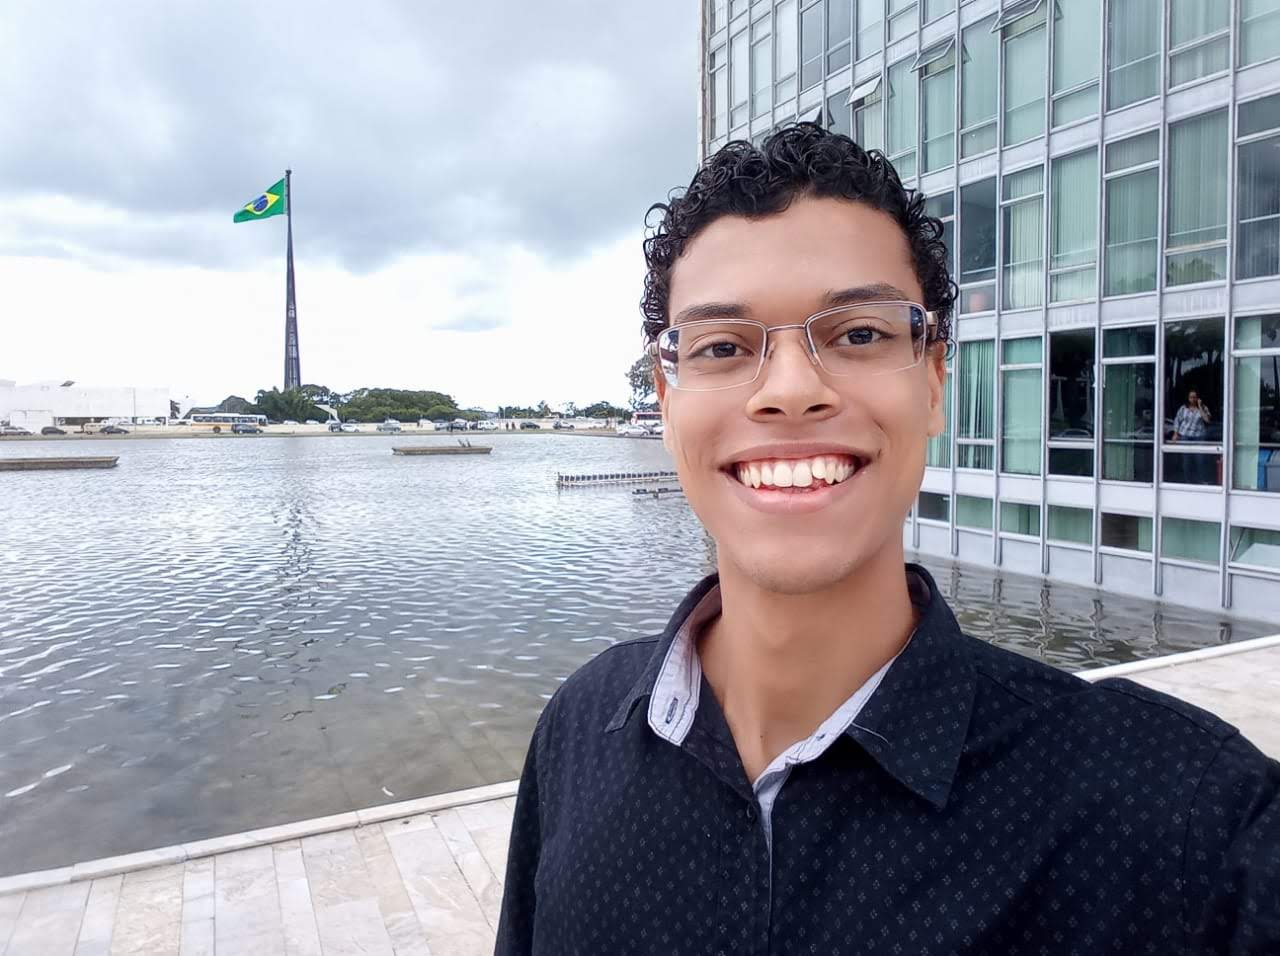
\includegraphics[width=\linewidth]{resources/perfil.jpeg}	%trimming relative to image size

%---------------------------------------------------------------------------------------
%	META SKILLS
%----------------------------------------------------------------------------------------
	\fcolorbox{white}{white}{\begin{minipage}[c][1.0cm][c]{1\mpwidth}
		\LARGE{\textbf{\textcolor{maincol}{Matheus Cardoso}}} \\[2pt]
		\normalsize{ \textcolor{maincol} {Computer Scientist (B. Sc.)} }
\end{minipage}}

\cvsection{Contact}

% \icontext{MapMarker}{16}{Street name XX\\D-XXXXX Lorem}{black}\\[6pt]
\icontext{MobilePhone}{16}{+55 (61) 98264-5973}{black}\\[3pt]
\iconemail{Envelope}{16}{cardosaum@pm.me}{cardosaum@pm.me}{black}\\[3pt]
% \iconhref{Home}{16}{XXX.XXX-XXXX.XX}{http://XXX-XXX.XXX.XX}{black}\\[6pt]
\iconhref{Github}{16}{cardosaum}{https://www.github.com/cardosaum}{black}\\[3pt]
\iconhref{Linkedin}{16}{matheus-c-souza}{https://www.linkedin.com/in/matheus-c-souza}{black}\\[3pt]
\iconhref{Home}{16}{mcscv.netlify.com}{https://www.linkedin.com/in/matheus-c-souza}{black}\\[3pt]
% \iconhref{Xing}{16}{xing.com/user\_name}{https://www.xing.com/profile/User_Name}{black}\\


% \icontext{CaretRight}{12}{05.03.1999 in São Paulo}{black}\\[6pt]
% \icontext{CaretRight}{12}{Brazilian}{black}\\[6pt]
% \icontext{CaretRight}{12}{Unmarried}{black}\\[6pt]


%%%%%%%%
\cvsectionskill{Skills}

%%%%
\cvsectionsmall{Programming \\ Languages}

\cvskill{Python} {3+ yrs.} {0.6}

\cvskill{Shell Scripting} {3+ yrs.} {0.6}

\cvskill{R} {1.5+ yrs.} {0.30}

\cvskill{C/C++} {1+ yrs.} {0.20}

\cvskill{SQL} {6+ mos.} {0.10}

\cvskill{Java} {6+ mos.} {0.10}

\cvskill{Rust} {6+ mos.} {0.10}

\cvskill{Javascript} {6+ mos.} {0.10}

\cvskill{RISC-V Assembly} {6+ mos.} {0.10}
%%%%

%%%%
\cvsectionsmall{Technologies}

\cvskill{HTML/CSS} {2.5+ yrs.} {0.50}

\cvskill{Git} {2.5+ yrs.} {0.50}

\cvskill{\LaTeX} {1.5+ yrs.} {0.30}
\vfill\null
%%%%

%%%%
\cvsectionsmall{Frameworks}

\cvskill{Biopython} {2.5+ yrs.} {0.50}

\cvskill{Tidyverse} {1.5+ yrs.} {0.30}

\cvskill{Tidymodels} {1.5+ yrs.} {0.30}

\cvskill{Numpy} {6+ mos.} {0.10}

\cvskill{Pandas} {6+ mos.} {0.10}

\cvskill{Django} {6- mos.} {0.06}
%%%%


%%%%
\cvsectionsmall{Areas of expertise}

\cvskill{System administration/ \newline Linux} {3+ yrs.} {0.6}

\cvskill{Bioinformatics} {2.5+ yrs.} {0.5}

\cvskill{Data science} {2+ yrs.} {0.4}

\cvskill{Low level programming/ \newline Assembly} {6+ mos.} {0.10}
%%%%


%%%%
\cvsectionsmall{Languages}

\cvskill{Portuguese} {Native} {1}

\cvskill{English} {B2} {0.66}

\cvskill{Spanish} {B1} {0.50}
%%%%

%%%%%%%%

% \newpage
% %---------------------------------------------------------------------------------------
% %	EDUCATION
% %----------------------------------------------------------------------------------------
% \cvsection{Education}

% \cvmetaevent
% {01/2021 - Present}
% {Computer Science (B.Sc.)}
% {University of Brasília - UnB}

% \cvmetaevent
% {01/2020 - 12/2020}
% {Computer Science (B.Sc.)}
% {Federal University of Rio de Janeiro - UFRJ}
% {\footnotesize Note: Opted to change university due to COVID pandemic}

% \cvmetaevent
% {01/2019 - 12/2019}
% {Biotechnology (B.Sc.)}
% {University of Brasília - UnB}
% {\footnotesize Note: Opted to change university due to preference for programming}



% \cvsection{Projects}

% 	\href{https://github.com/cardosaum/attila}{\textbf{Attila}}\\ AutomaTed Tool For Immunoglobulin Analysis, A software to assess monoclonal antibody enrichment.\\

% 	\href{https://github.com/cardosaum/isc-lolo-game}{\textbf{The Adventures of Lolo}}\\ Remake of the game \textit{The Adventures of Lolo} in RISC-V assembly.\\

% 	\href{https://github.com/cardosaum/ufrj-comp1-senha}{\textbf{Mastermind}}\\ Remake of the game \textit{Mastermind} in C.\\


\cvsection{Interests}

\icontext{CaretRight}{12}{Bioinformatics/\\Computational Biology}{black}\\[6pt]
\icontext{CaretRight}{12}{Artificial Intelligence}{black}\\[6pt]
\icontext{CaretRight}{12}{Protein Folding}{black}\\[6pt]
\icontext{CaretRight}{12}{Open Source}{black}\\[6pt]
\icontext{CaretRight}{12}{Embedded Systems}{black}\\[6pt]

% \vfill
% \mbox{}
% \vfill
% \mbox{}
% \vfill
% \mbox{}
% \vfill
% \mbox{}
% \vfill
% \mbox{}
% \vfill
% \mbox{}
% \vfill
% \mbox{}
% \vfill
% \mbox{}
% \vfill
% \mbox{}
% \vfill
% \mbox{}
% \vfill
% \mbox{}
% \vfill
% \mbox{}
% \vfill
% \mbox{}


% \cvqrcode{0.3}

\end{leftcolumn}
\begin{rightcolumn}
%---------------------------------------------------------------------------------------
%	TITLE  HEADER
%----------------------------------------------------------------------------------------


%---------------------------------------------------------------------------------------
%	PROFILE
%----------------------------------------------------------------------------------------
\cvsection{Biography}
\vspace{4pt}

\cvtext{

  Computer science student, work with data analysis in the area of genomics and
  proteomics, developing software that automatically generates statistics on
  enriched monoclonal antibodies. His work mainly involves machine learning
  techniques, data mining, data analysis and data visualization. As a result, in
  addition to working in the area of computer sciences, he also have a strong
  focus on biological and data sciences.\\[-8pt]

  In his free time he have been contributing to open source projects as well; Spanning from data science frameworks (\href{https://pandas.pydata.org/}{Pandas}), to educational learning software (\href{https://apps.ankiweb.net/}{Anki}), and productivity programs (\href{https://github.com/hrkfdn/ncspot/}{ncspot}, \href{https://github.com/Airblader/unclutter-xfixes/issues/67}{unclutter} and \href{https://github.com/Cardosaum/hacksaw/}{hacksaw}).
  % \Blindtext[1]


}


%---------------------------------------------------------------------------------------
%	WORK EXPERIENCE
%----------------------------------------------------------------------------------------

\vspace{10pt}
\cvsection{Education}
\vspace{4pt}


\cvevent
{03/2021 - today}
	{Computer Science | B.Sc. student}
	{University of Brasília - UnB}
	{I aced all my exams and projects until now.\\[5]GPA: 5/5}
	% {I don't have much to say yet.\\[5]GPA: 4.8/5}
	\vfill\null


\cvevent
{01/2020 - 03/2021}
	{Computer Science | B.Sc. student}
	{Federal University of Rio de Janeiro - UFRJ}
	{Due to the pandemic I opted to move from Rio back to Brasília.\\[5]GPA: 2.9/5}
	\vfill\null

	
\cvevent
{01/2019 - 12/2019}
	{Biotechnology | B.Sc. student}
	{University of Brasília - UnB}
	{I had the opportunity to internship in UnB's Bioinformatics and Immunology
	  laboratory, where I contributed to the development of a software to assess
	  enrichment of monoclonal antibodies. There I found that more than research
	  I really enjoy to code, so I opted to change my majors to Computer
	  Science.\\[5]GPA: 4.8/5}
	\vfill\null


\cvsection{Projects}

\cvevent
{01/2019 - today}
	{\href{https://github.com/cardosaum/attila}{\textbf{ATTILA - AutomaTed Tool For Immunoglobulin}}}
	{University of Brasília - UnB}
	{ATTILA is an open source project that analyses phage display libraries in
    order to assess monoclonal antibody enrichment. Doing this, the software is
    able to predict which antibodies can more effectively bind to target
    molecules. As a result, ATTILA becomes a useful tool to scientists working
    on vaccine development.} \vfill\null

  \cvevent {06/2021 - today}
  {\href{https://github.com/cardosaum/cdr3-parser}{\textbf{cdr3-parser}}}
  {University of Brasília - UnB}
  {\textbf{cdr3-parser} is a command line program
    written in \texttt{Rust} to convert intermediate output files generated from
    ATTILA into \texttt{csv} files containing statistics about VH-CDR3 regions
    presented in the input file. \textbf{cdr3-parser} leverages \texttt{Rust}'s
    thread-safe capabilities to parse the file in the most efficiente way
    possible using all threads available in the UnB's Bioinformatics laboratory
    server.} \vfill\null


\cvevent
{03/2021 - 05/2021}
	{\href{https://github.com/cardosaum/isc-lolo-game}{\textbf{The Adventures of Lolo}}}
	{University of Brasília - UnB}
	{Remake of the game \textit{The Adventures of Lolo} in \texttt{RISC-V Assembly}.}
	\vfill\null


\cvevent
{02/2021 - 03/2021}
	{\href{https://github.com/cardosaum/ufrj-comp1-senha}{\textbf{Mastermind}}}
	{Federal University of Rio de Janeiro - UFRJ}
	{Remake of the game \textit{Mastermind} in \texttt{C}.}
  \vfill\null

\cvevent
{08/2020}
	{\href{https://cardosaum.shinyapps.io/Matheus-Cardoso-DDP-JHU-Week4}{\textbf{Brazilian Students' Performance on ENEM}}}
	{Johns Hopkins Bloomberg School of Public Health}
	{A data visualization project showing the performance of Brazilian students applying to a bachelors of science at Universidade de São Paulo (USP), one of the best universities in Brazil.}
  \vfill\null

\cvevent
{08/2020}
	{\href{https://cardosaum.shinyapps.io/WordPredictor_Final_Project_JHU_Matheus_C}{\textbf{Word Predictor Model}}}
	{Johns Hopkins Bloomberg School of Public Health}
	{A web application powered by a machine learning model able to predict the next word in a sentence.}
  \vfill\null


\cvsection{Awards \& Certificates}

\cvevent
{01/2020 - 09/2020}
	{\href{https://www.coursera.org/account/accomplishments/specialization/certificate/JTYMU3V78XWZ}{\textbf{Data Science Specialization}}}
	{Johns Hopkins Bloomberg School of Public Health}
	{}
	\vfill\null

\cvevent
{2020}
	{\textbf{Copenhagen Bioinformatics Hackathon}}
	{BioLib}
	{Winner of the Hackathon challenge \textit{``Variant Pathogenicity Prediction''}.}
	\vfill\null

\cvevent
{2019}
	{\href{https://talentouniversitario.capes.gov.br/#!/index}{\textbf{Capes Prize University Talent}}}
	{CAPES}
	{Awarded by the Brazilian Ministry of Education as one of the top 1000 most talented freshman students in the country.}
	\vfill\null

\cvevent
{2019}
	{Hackathon NASA Space Apps BSB}
	{NASA}
	{Awarded as 5th out of 60+ teams in the Brazil's Midwest regional phase.}
	\vfill\null


% \cvsection{Service}

% \cvevent
% {2019}
% 	{CPA}
% 	{NASA}
% 	{Awarded as 5th out of 60+ teams in the Brazil's Midwest regional phase.}
% 	\vfill\null

% \cvevent
% {03/2020 - 09/2020}
% 	{\href{https://www.coursera.org/account/accomplishments/specialization/certificate/JTYMU3V78XWZ}{\textbf{Data Science Specialization}}}
% 	{Johns Hopkins Bloomberg School of Public Health}
% 	{}
% 	\vfill\null



% \cvsection{Publications}

% \item Author, G. \& Author, P. \&  Author G. (2020). "This is the title of the publication". In: \textit{Proceedings of the 28th Conference on Lipsum (LIPSUM)}, Lipsum, June 12-17, 2020.
% \item Author, G. \& Author, P. \&  Author G. (2020). "This is the title of the publication". In: \textit{Proceedings of the 28th Conference on Lipsum (LIPSUM)}, Lipsum, June 12-17, 2020.
% \item Author, G. \& Author, P. \&  Author G. (2020). "This is the title of the publication". In: \textit{Proceedings of the 28th Conference on Lipsum (LIPSUM)}, Lipsum, June 12-17, 2020.
% \end{itemize}

% % hofixes to create fake-space to ensure the whole height is used
\mbox{}
\vfill
\mbox{}
\vfill
\mbox{}
\vfill
\mbox{}
\vfill
\mbox{}
\vfill
\mbox{}
\vfill
\mbox{}
\vfill
\mbox{}
\vfill
\mbox{}
\vfill
\mbox{}
\vfill
\mbox{}


São Paulo, \today \hspace{1cm} \hrulefill

\hspace*{30mm}\phantom{Lorem, \today }Matheus Cardoso de Souza

\end{rightcolumn}
\end{paracol}


\end{document}
